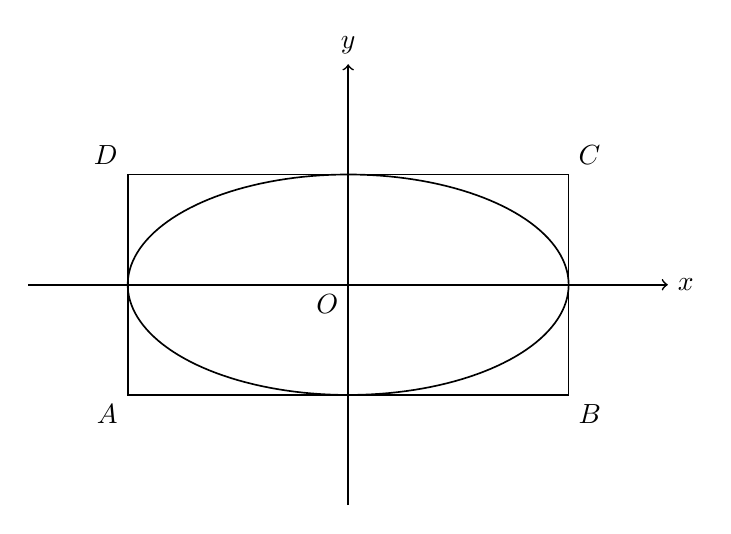
\begin{tikzpicture}[line width=.6pt]
  % exact: ellipse x^2/4+y^2=1, rectangle [-2,2]x[-1,1], scale 1.4
  \begin{scope}[scale=1.4]
    % axes
    \draw[->] (-2.9,0) -- (2.9,0);
    \draw[->] (0,-2.0) -- (0,2.0);
    % rectangle ABCD
    \draw (-2,-1) rectangle (2,1);
    % ellipse from formula
    \draw plot[domain=0:360, samples=160] ({2*cos(\x)},{sin(\x)});
    % labels
    \node[anchor=west] at (2.9,0) {$x$};
    \node[anchor=south] at (0,2.0) {$y$};
    \node[anchor=north east] at (0,0) {$O$};
    \node[anchor=north east] at (-2,-1) {$A$};
    \node[anchor=north west] at (2,-1) {$B$};
    \node[anchor=south west] at (2,1) {$C$};
    \node[anchor=south east] at (-2,1) {$D$};
  \end{scope}
\end{tikzpicture}
